\documentclass[tikz,border=2pt]{standalone}
\usepackage{amsmath}
\usetikzlibrary{arrows.meta,decorations.pathreplacing}
\begin{document}
% Random sums inherit the order of their ingredients: if severities X_i <= Y_i and counts M <= N in the same
% order (st, sl or e), with severities nonnegative, i.i.d. and independent of the counts, then sum_{i<=M} X_i <= sum_{i<=N} Y_i.
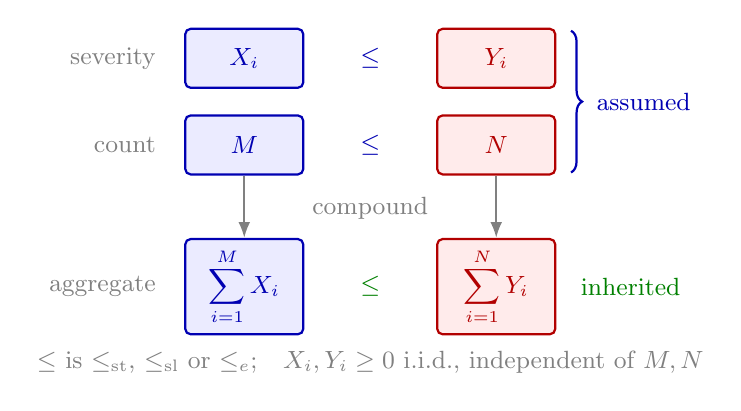
\begin{tikzpicture}[font=\small, >={Latex[length=2mm]},
  bx/.style={draw, thick, rounded corners=2pt, minimum width=1.5cm, minimum height=0.75cm}]
  \def\xl{0} \def\xr{3.2}
  % row labels
  \node[gray, anchor=east] at (-1.0,0) {severity};
  \node[gray, anchor=east] at (-1.0,-1.1) {count};
  \node[gray, anchor=east] at (-1.0,-2.9) {aggregate};
  % X side (left column) and Y side (right column)
  \node[bx, blue!70!black, fill=blue!8] (x) at (\xl,0) {$X_i$};
  \node[bx, blue!70!black, fill=blue!8] (m) at (\xl,-1.1) {$M$};
  \node[bx, blue!70!black, fill=blue!8, minimum height=1.05cm] (sx) at (\xl,-2.9) {$\displaystyle\sum_{i=1}^{M}X_i$};
  \node[bx, red!70!black, fill=red!8] (y) at (\xr,0) {$Y_i$};
  \node[bx, red!70!black, fill=red!8] (n) at (\xr,-1.1) {$N$};
  \node[bx, red!70!black, fill=red!8, minimum height=1.05cm] (sy) at (\xr,-2.9) {$\displaystyle\sum_{i=1}^{N}Y_i$};
  % compounding
  \draw[->, thick, gray] (m.south) -- (sx.north);
  \draw[->, thick, gray] (n.south) -- (sy.north);
  \node[gray] at (0.5*\xl+0.5*\xr,-1.9) {compound};
  % assumed and inherited orders
  \node[blue!70!black] at (0.5*\xl+0.5*\xr,0) {$\le$};
  \node[blue!70!black] at (0.5*\xl+0.5*\xr,-1.1) {$\le$};
  \node[green!50!black] at (0.5*\xl+0.5*\xr,-2.9) {$\le$};
  \draw[decorate, decoration={brace, amplitude=4pt}, thick, blue!70!black] (\xr+0.95,0.35) -- (\xr+0.95,-1.45);
  \node[blue!70!black, anchor=west] at (\xr+1.15,-0.55) {assumed};
  \node[green!50!black, anchor=west] at (\xr+0.95,-2.9) {inherited};
  % assumptions
  \node[gray, anchor=north] at (0.5*\xl+0.5*\xr,-3.6) {$\le$ is $\le_{\mathrm{st}}$, $\le_{\mathrm{sl}}$ or $\le_e$;\quad $X_i,Y_i\ge0$ i.i.d., independent of $M,N$};
\end{tikzpicture}
\end{document}
